\section{Durchführung und Aufbau}
\label{sec:Durchführung}
Da die Energieänderungen der Zeeman-Aufspaltung sehr gering sind, muss ein optisches Bauteil mit einem hohen Auflösungsvermögen verwendet werden. Dazu wird eine Lummer-Gehrcke-Platte verwendet, deren Funktionsweise im folgenden kurz skizziert wird.

\subsection{Lummer-Gehrcke-Platte}
Bei einer Lummer-Gehrcke-Platte wird Licht durch ein Prisma in eine Glasplatte mit planparallelen Flächen eingekoppelt. Das Licht wird an den Grenzflächen zu einem großen Teil reflektiert. Jedoch tritt ein geringer Teil der Strahlung aus der Platte aus. Durch justage der Lummer-Gehrcke-Platte wird versucht 10-14 konstruktive Interferenzmaxima in der Kamera abzubilden. Eine Skizze der Lummer-Gehrcke-Platte ist in Abbildung \ref{fig:Lum} zu sehen.

\begin{figure}[H]
  \centering
  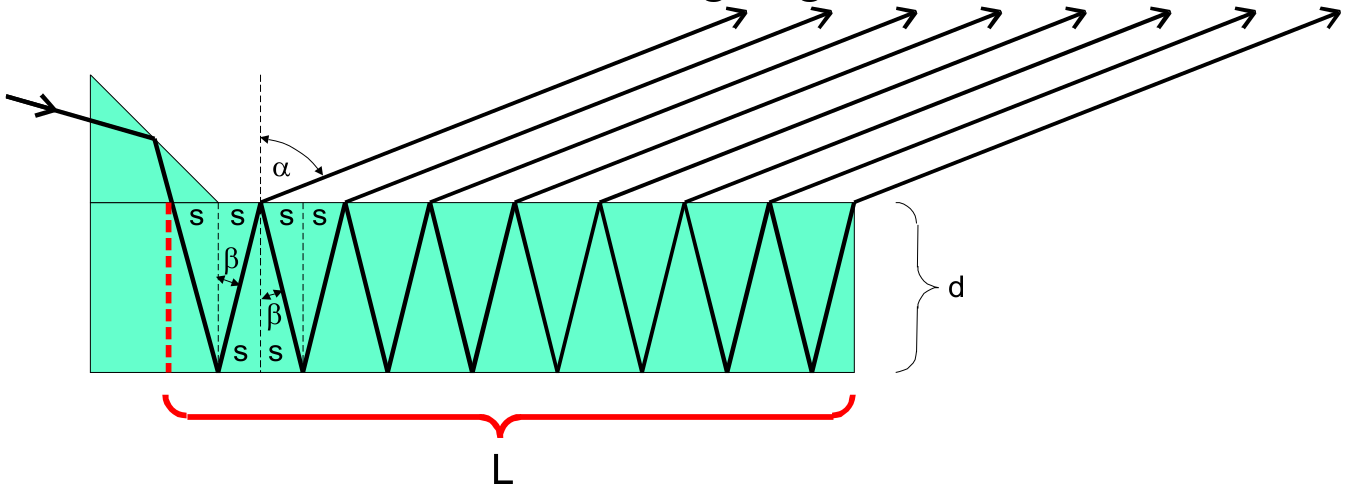
\includegraphics[height=6cm]{Bilder/Lummer.png}
  \caption{Funktionsweise einer Lummer-Gehrcke-Platte \cite{V27}}
  \label{fig:Lum}
\end{figure}

Die Strahlen interferieren Konstruktiv wenn sie die Gleichung
\begin{equation}
  2 d \cos(\alpha) = n \lambda
\end{equation}
erfüllen, wobei $d$ die Dicke der Platte ist. Der Gleichung kann entnommen werden, dass der Gangunterschied genau ein ganzzahliges vielfache der eingestrahlten Wellenlänge ist. Durch das einschalten eines Magnetfeldes beträgt die Wellenlängenändeung $\delta \lambda$ woraus eine Verschiebung der Interferenzstreifen von $\delta$s verursacht wird. Auf die Wellenlängenändeung wird in der Auswertung noch weiter eingegangen.

\subsection{Versuchsaufbau}
Für den Versuch befindet sich zwischen den Polschuhen des Magneten eine Cd-Lampe dessen Licht zunächst fokussiert und anschließend durch ein Gradsichtprisma geschickt wird. Anschließend wird das in Spektrallinien aufgespaltene Licht durch eine Polarisationsfilter geschickt, welcher dazu dient, den $\sigma$ vom $\pi$ Übergang zu unterscheiden. Mittels einer Linse werden die durch ein Gradsichtprisma in Spektralfarben zerlegten Linien, die nicht gewünschten werden, von der optischen Achse weggebrochen, sodass diese nicht mehr den dahinterstehenden Spalt passieren können.
\begin{figure}[H]
  \centering
  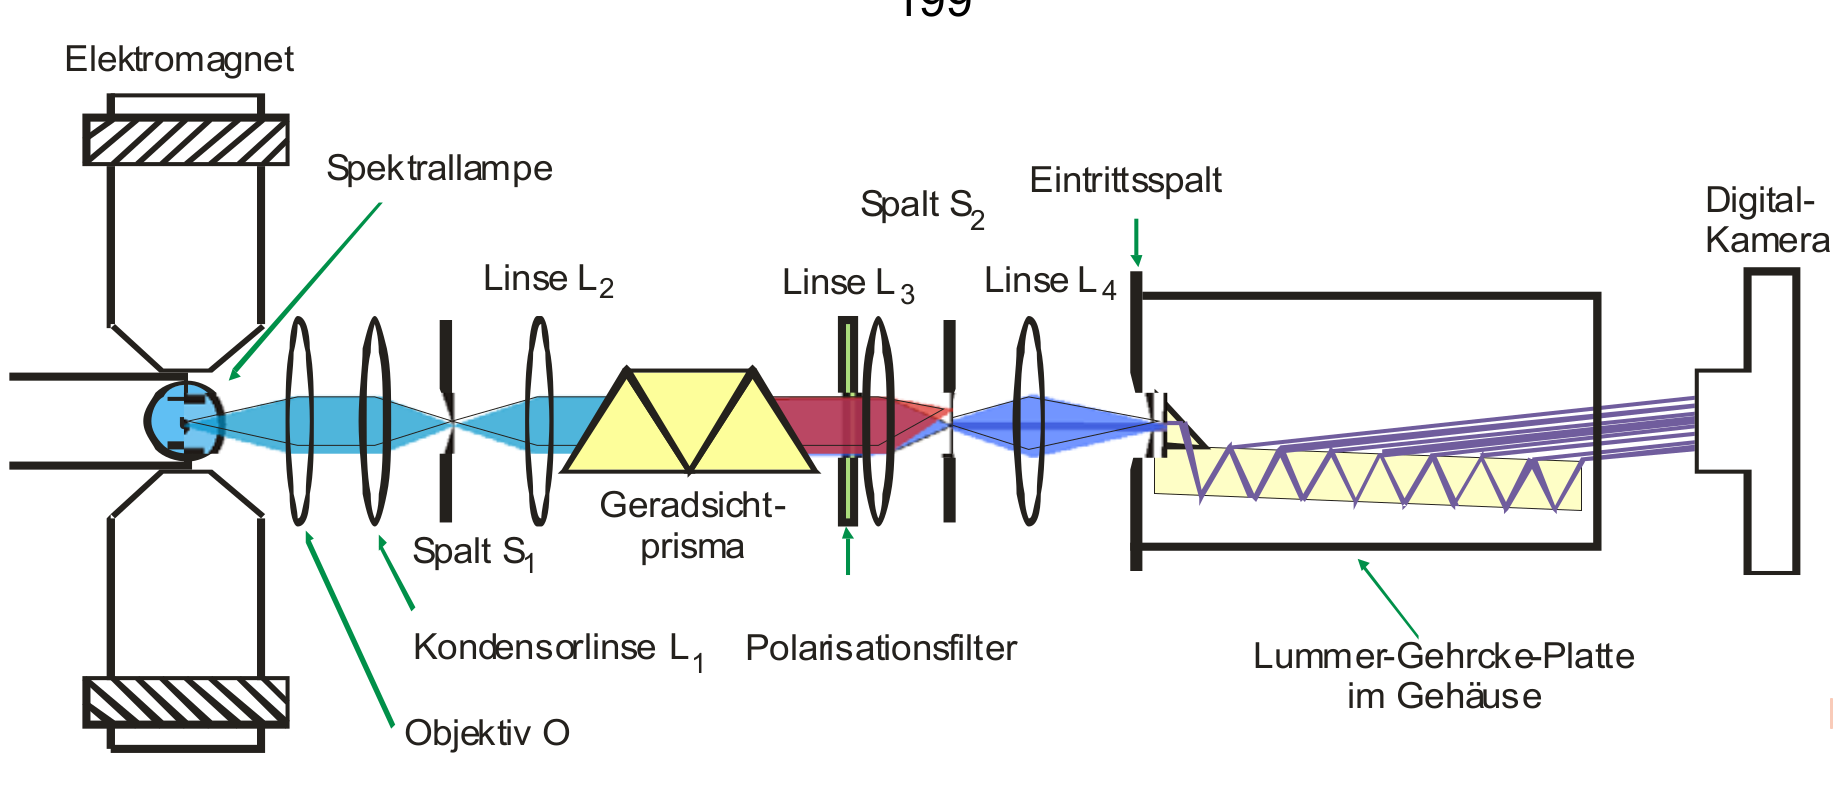
\includegraphics[height=6cm]{Bilder/Aufbau.png}
  \caption{Aufbau der Messaperatur \cite{V27}}
\end{figure}
Hinter dem Spalt wird eine weiter Linse aufgestellt, um den Strahlengang auf die Eintrittsöffnung der Lummer-Gehrcke-Platte scharf abzubilden. Zuletzt wird mittels einer Digitalkamera ein Foto von dem Interferenzbild aufgenommen.

\subsection{Durchführung}
Zuerst werden die optischen Bauteile in den Strahlengang gebracht und nacheinander ausgerichtet. Sofern dieses geschehen ist wird die Lummer-Gehrcke-Platte so ausgerichtet, dass das Interferenzbild in der Kamera zu sehen ist. Dabei ist darauf zu achten, dass der Fokus der Kamera angepasst wird, um ein scharfes Bild zu erhalten. Es werden zwei Bilder für die rote und drei für die blaue Spektrallinie geschossen. Zunächst wird ein Bild der Spektrallinie ohne äußeres B-Feld und anschließend zwei Bilder mit angelegtem B-Feld für beide Polarisationsrichtungen geschossen. Zuletzt wird eine Hysteresekurve des Magnetfeldes aufgenommen, wobei darauf zu achten ist, dass die Hallsonde möglichst nah an die Cd-Lampe zu halten ist um möglichst genau das B-Feld zu approximieren, welches die Lampe durchsetzt.
